\chapter{Example: Lomuto Partitioning Algorithm}\label{chapter:example}

As an example application of our refinement procedure, we implement the Lomuto partitioning algorithm naively \parencite[p.287]{bentley1984programming}, except that instead of having the pivot element at the end, we put it into the first place of the list (\autoref{fig:lomuto_impl}). The implementation is naive, because it simply replaces the arrays in the imperative implementation with functional lists, using the same operations. Due to that, the runtime of the algorithm increases from $\mathcal{O}(n)$ to $\mathcal{O}(n^2)$.

\begin{figure}[htbp]
    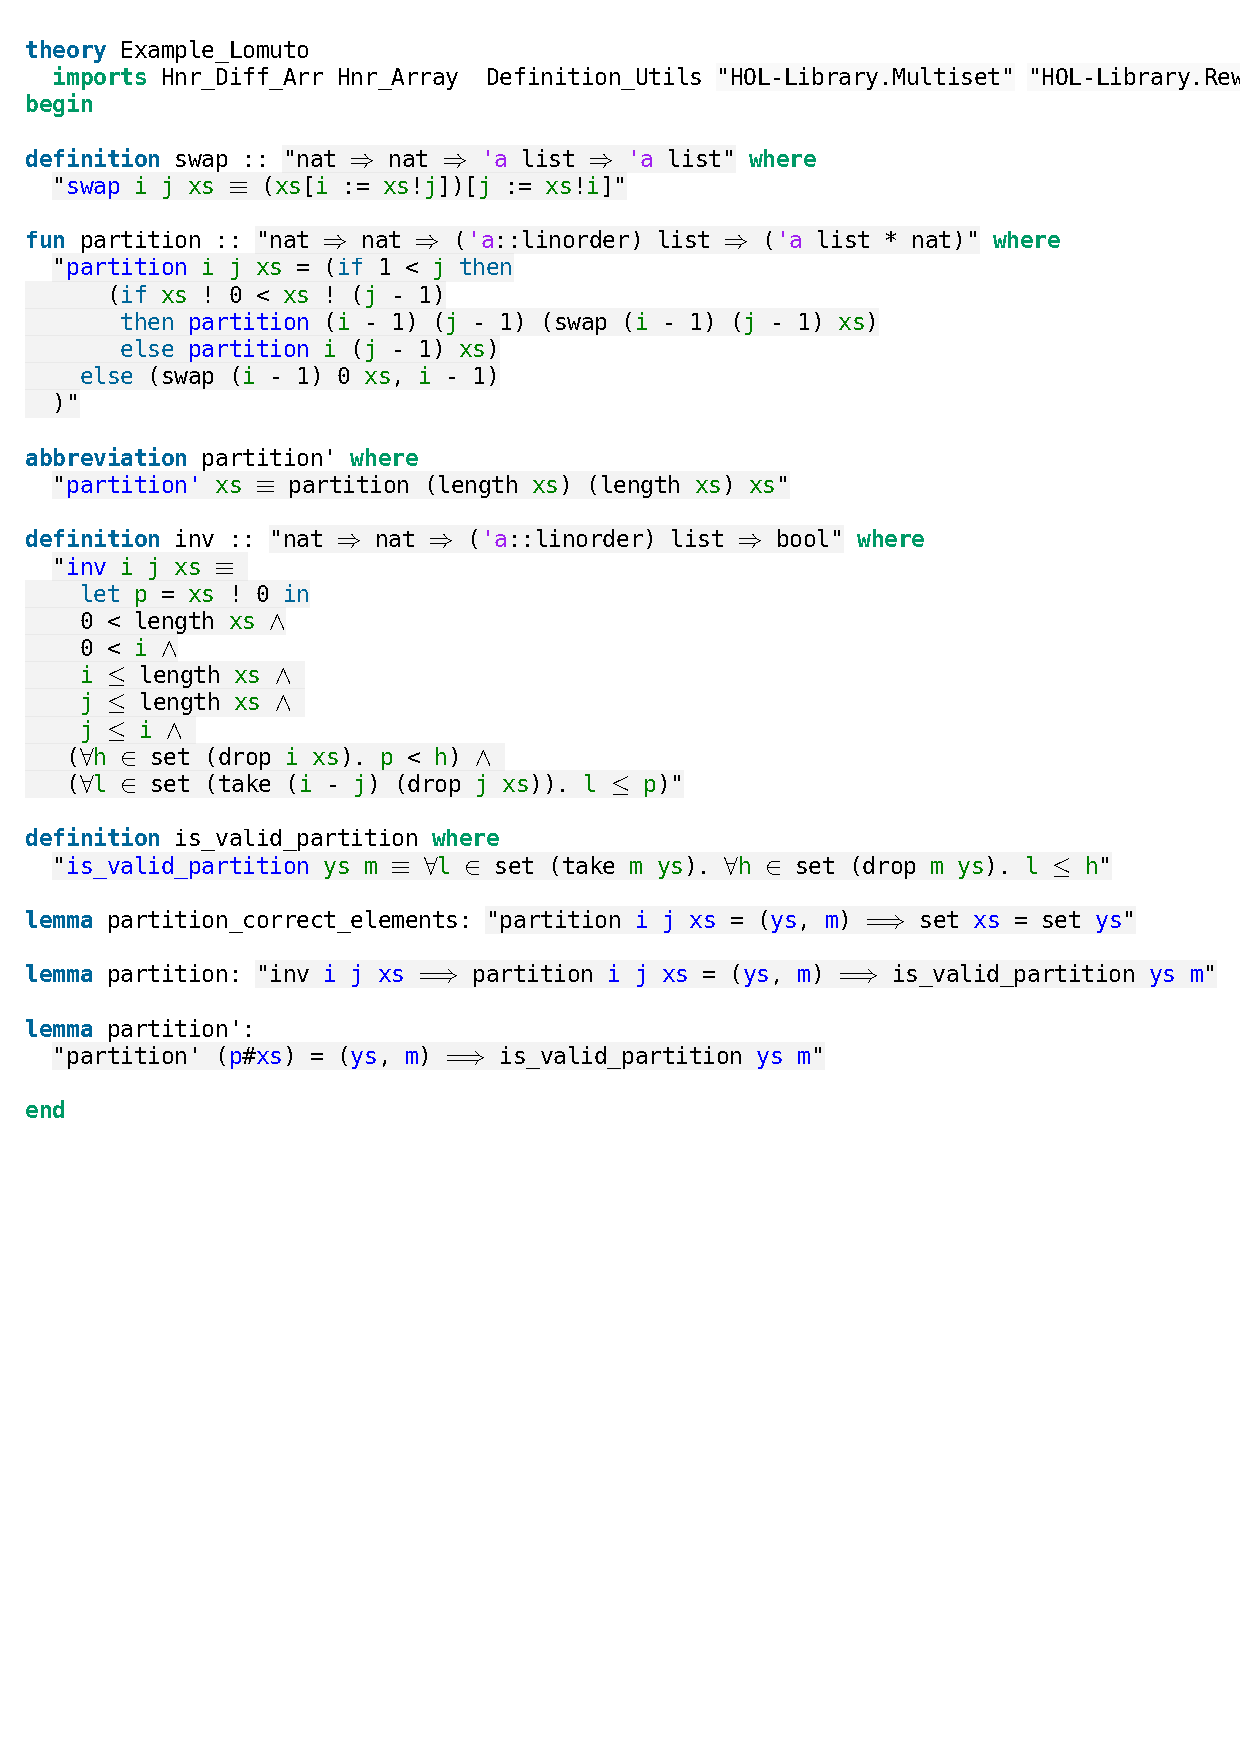
\includegraphics[trim={0 21cm 0 2,4cm}, clip, width=1.00\textwidth]{figures/Theory_Example_Lomuto_Impl.pdf}
    \caption[Naive Lomuto partitioning algorithm]{Naive Lomuto partitioning algorithm}
    \label{fig:lomuto_impl}
\end{figure}

\noindent By recursing on the list and returning a separate list per partition, like in the Isabelle standard library \parencite{list}, we can also reach a runtime in $\mathcal{O}(n)$. But it is not possible to reach the same runtime for every algorithm compared to its imperative counterpart when implemented purely functionally, since some have a logarithmic slowdown \parencite[p.108]{Pippenger_1997}.\\
With our refinement procedure, we do not need to rewrite the algorithm and still regain a runtime in $\mathcal{O}(n)$ for the Lomuto partitioning. As a first step for that, we verified the implementation by finding the invariant and doing a structural induction (\autoref{fig:lomuto_verification}).

\begin{figure}[htbp]
    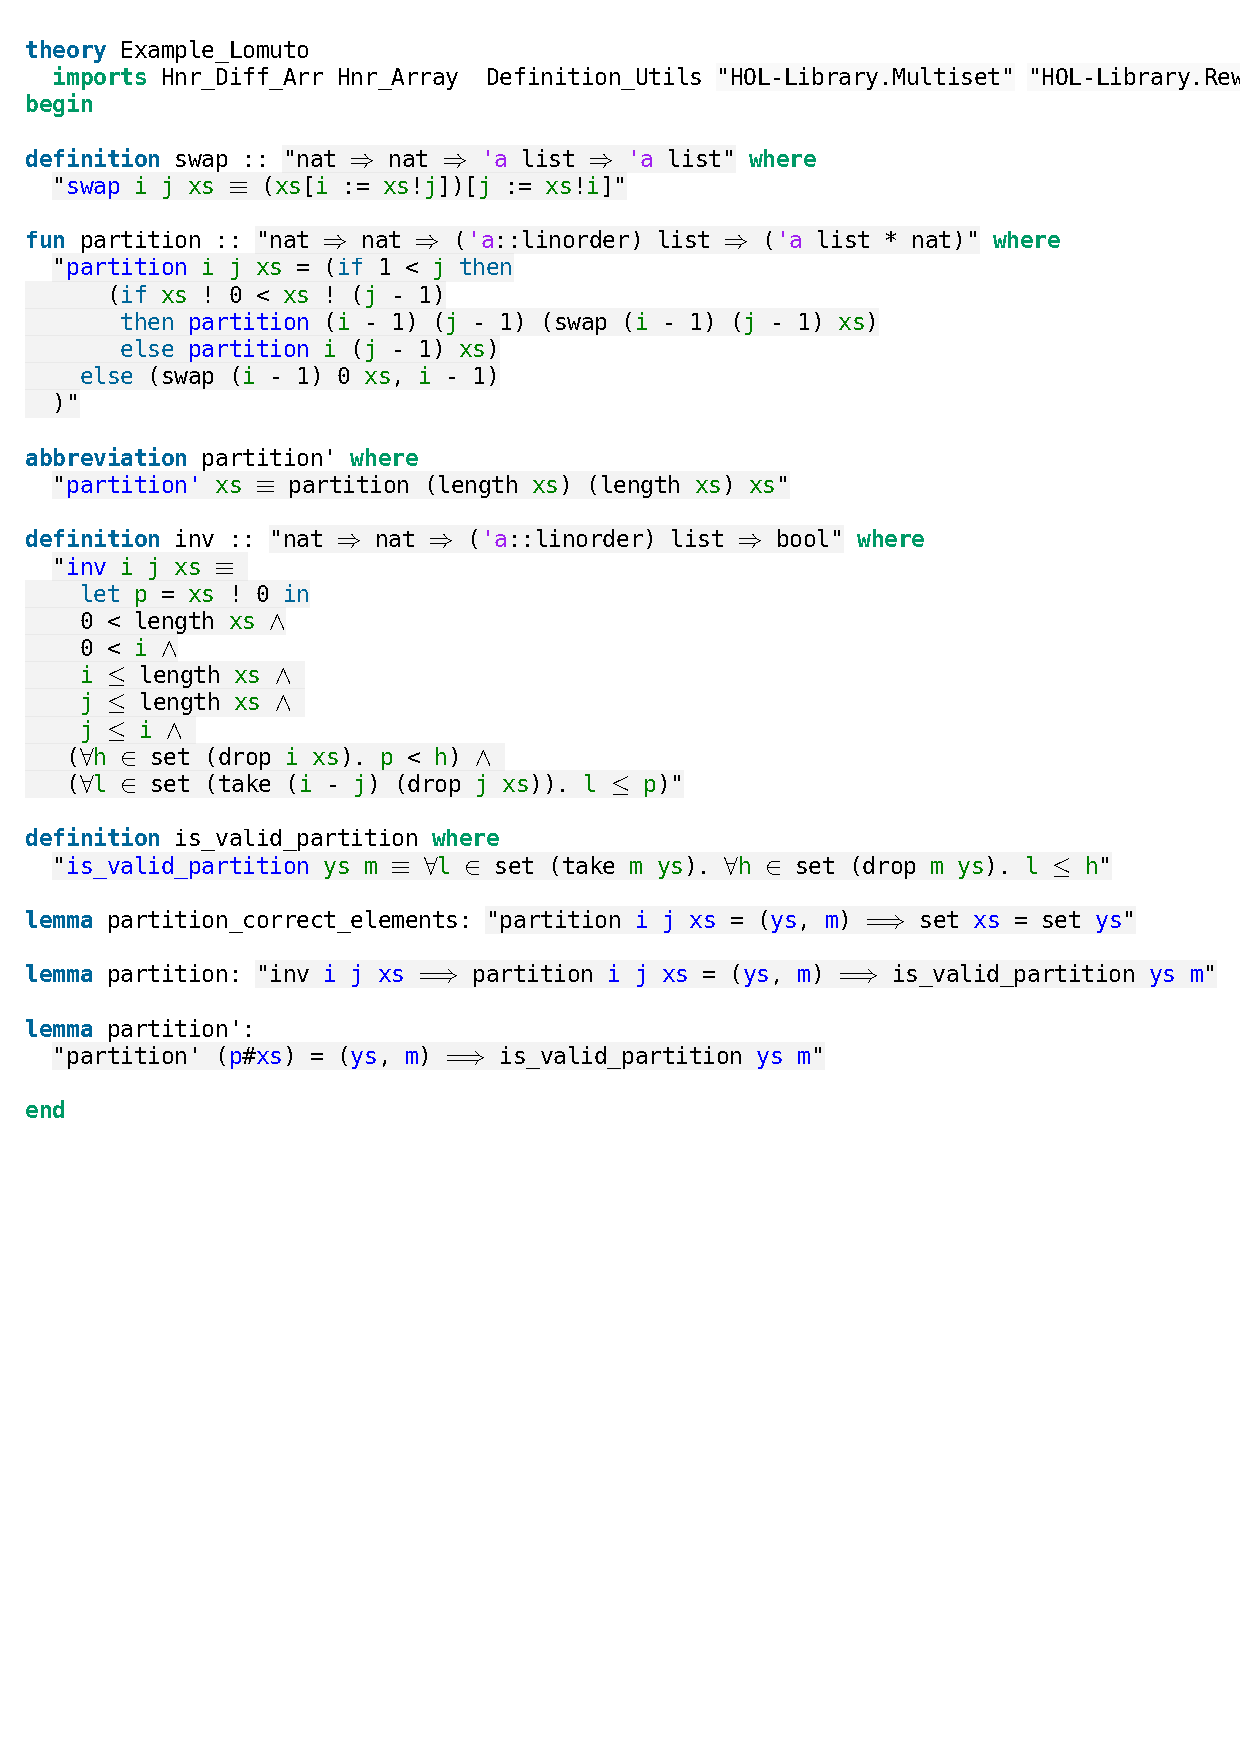
\includegraphics[trim={0 11,4cm 0 8,9cm}, clip, width=1.00\textwidth]{figures/Theory_Example_Lomuto_Impl.pdf}
    \caption[Verification of the naive Lomuto partitioning algorithm]{Verification of the naive Lomuto partitioning algorithm}
    \label{fig:lomuto_verification}
\end{figure}

\noindent Next, we need to monadify the implementation (see \autoref{chapter:automatic-refinement}). For now, we do this manually (\autoref{chapter:future_work}). Additionally, we verified that the monadified algorithm does the same as the original one. The monadified version of |swap| is in \autoref{fig:swap_opt} and the whole monadified algorithm is in \cite{repo}.

\begin{figure}[htbp]
    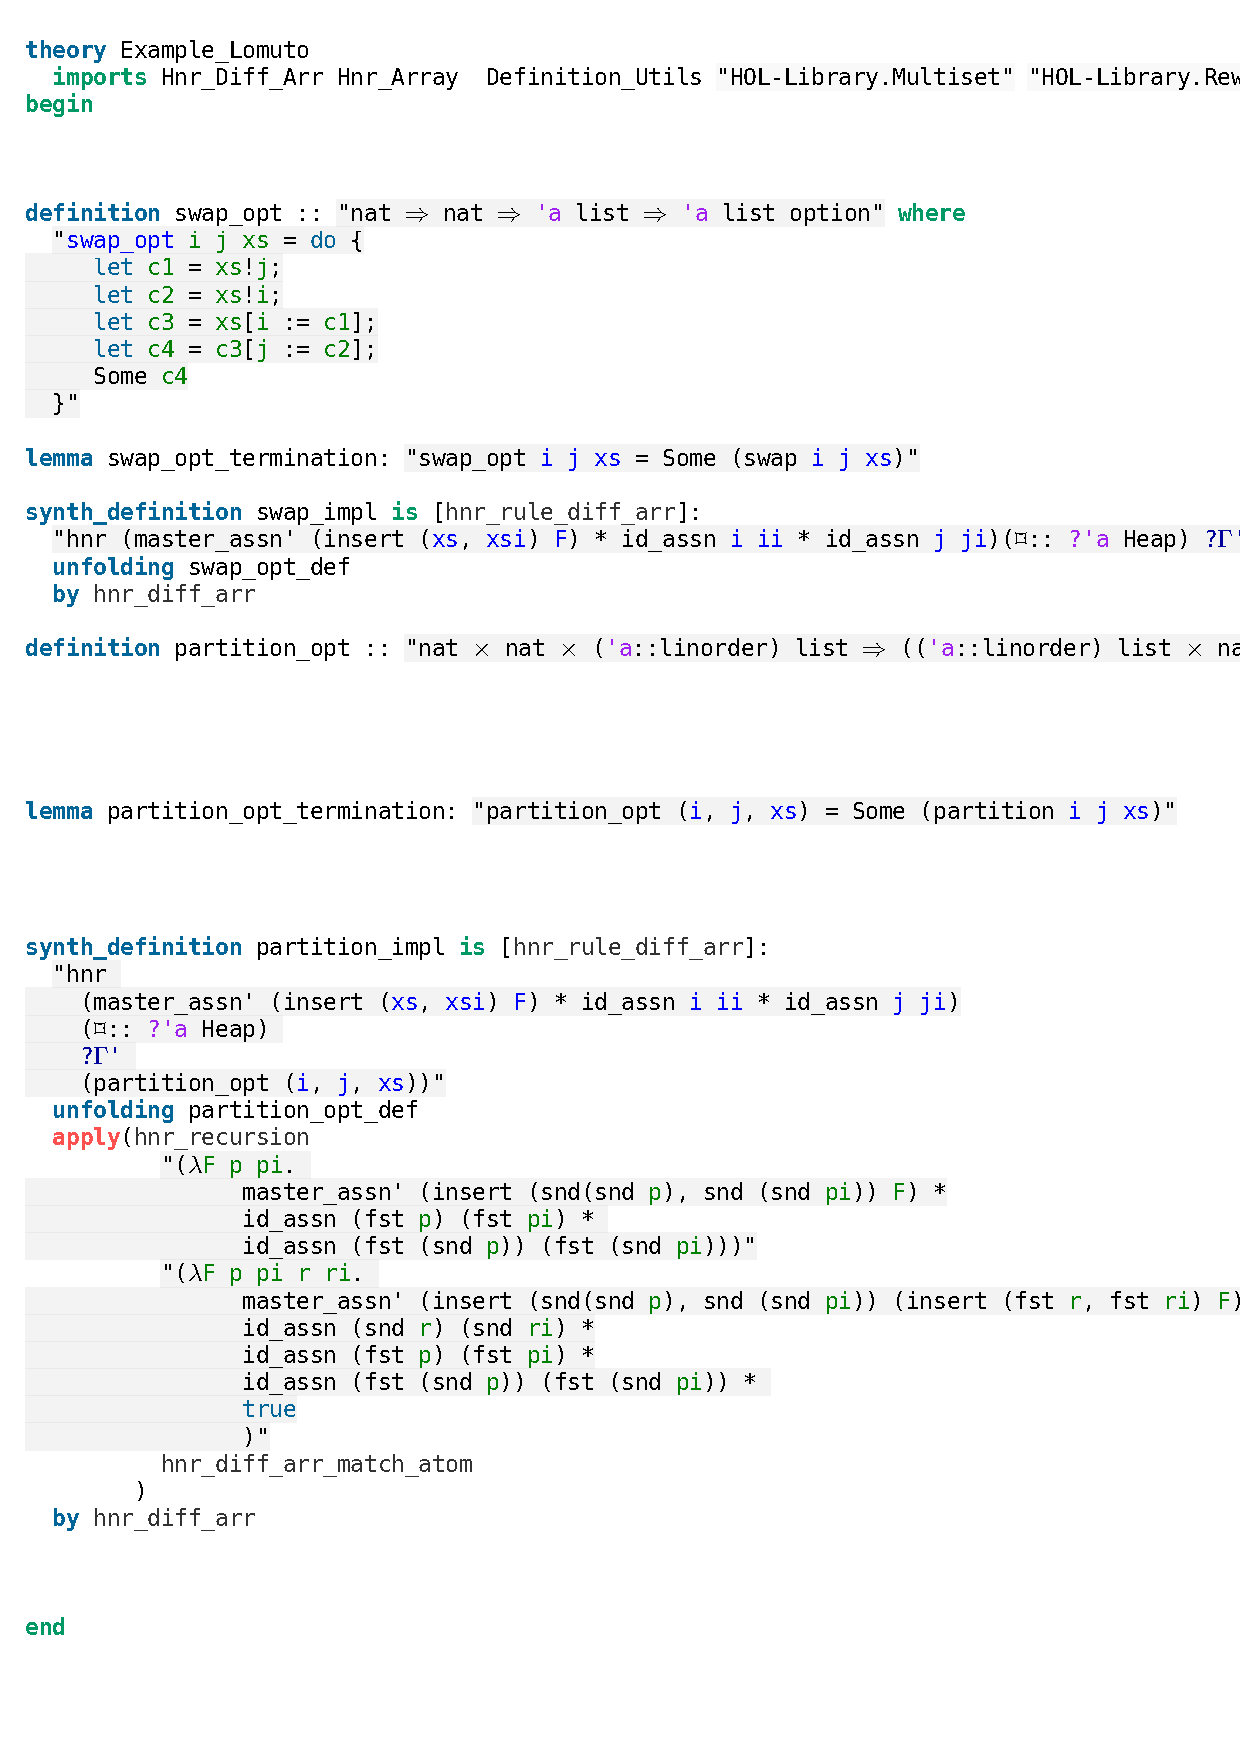
\includegraphics[trim={0 21,7cm 0 3,4cm}, clip, width=1.00\textwidth]{figures/Theory_Example_Lomuto_Translatiopn.pdf}
    \caption[Monadified swap implementation]{Monadified swap implementation}
    \label{fig:swap_opt}
\end{figure}

\noindent Now, we can start with the actual refinement process. The algorithm can be refined using arrays and diff arrays since the utilized list is used linearly. But if we change, for example, the order of the bindings of |c2| and |c3| in \autoref{fig:swap_opt}, the list would not be used linearly anymore and we would need a diff array.\\
The implementation of |swap| can be refined directly using the |hnr|\_|diff|\_|arr| method (\autoref{fig:hnr_diff_arr_method}). For |partition|, we first need to apply the recursion method (\autoref{section:hnr_recursion}) and supply the pre- and postcondition of the recursive calls in form of separation logic assertions (\autoref{fig:lomuto_ref}). They are straightforward and state that the parameters of the function as well as the result of the recursive calls are either identical to their refinements or in the case of the list it is refined to the respective diff array. Finally, our diff array refinement method (\autoref{fig:hnr_diff_arr_method}) can do the rest of the refinement automatically and replaces the list with diff arrays and its corresponding operations.

\begin{figure}[htbp]
    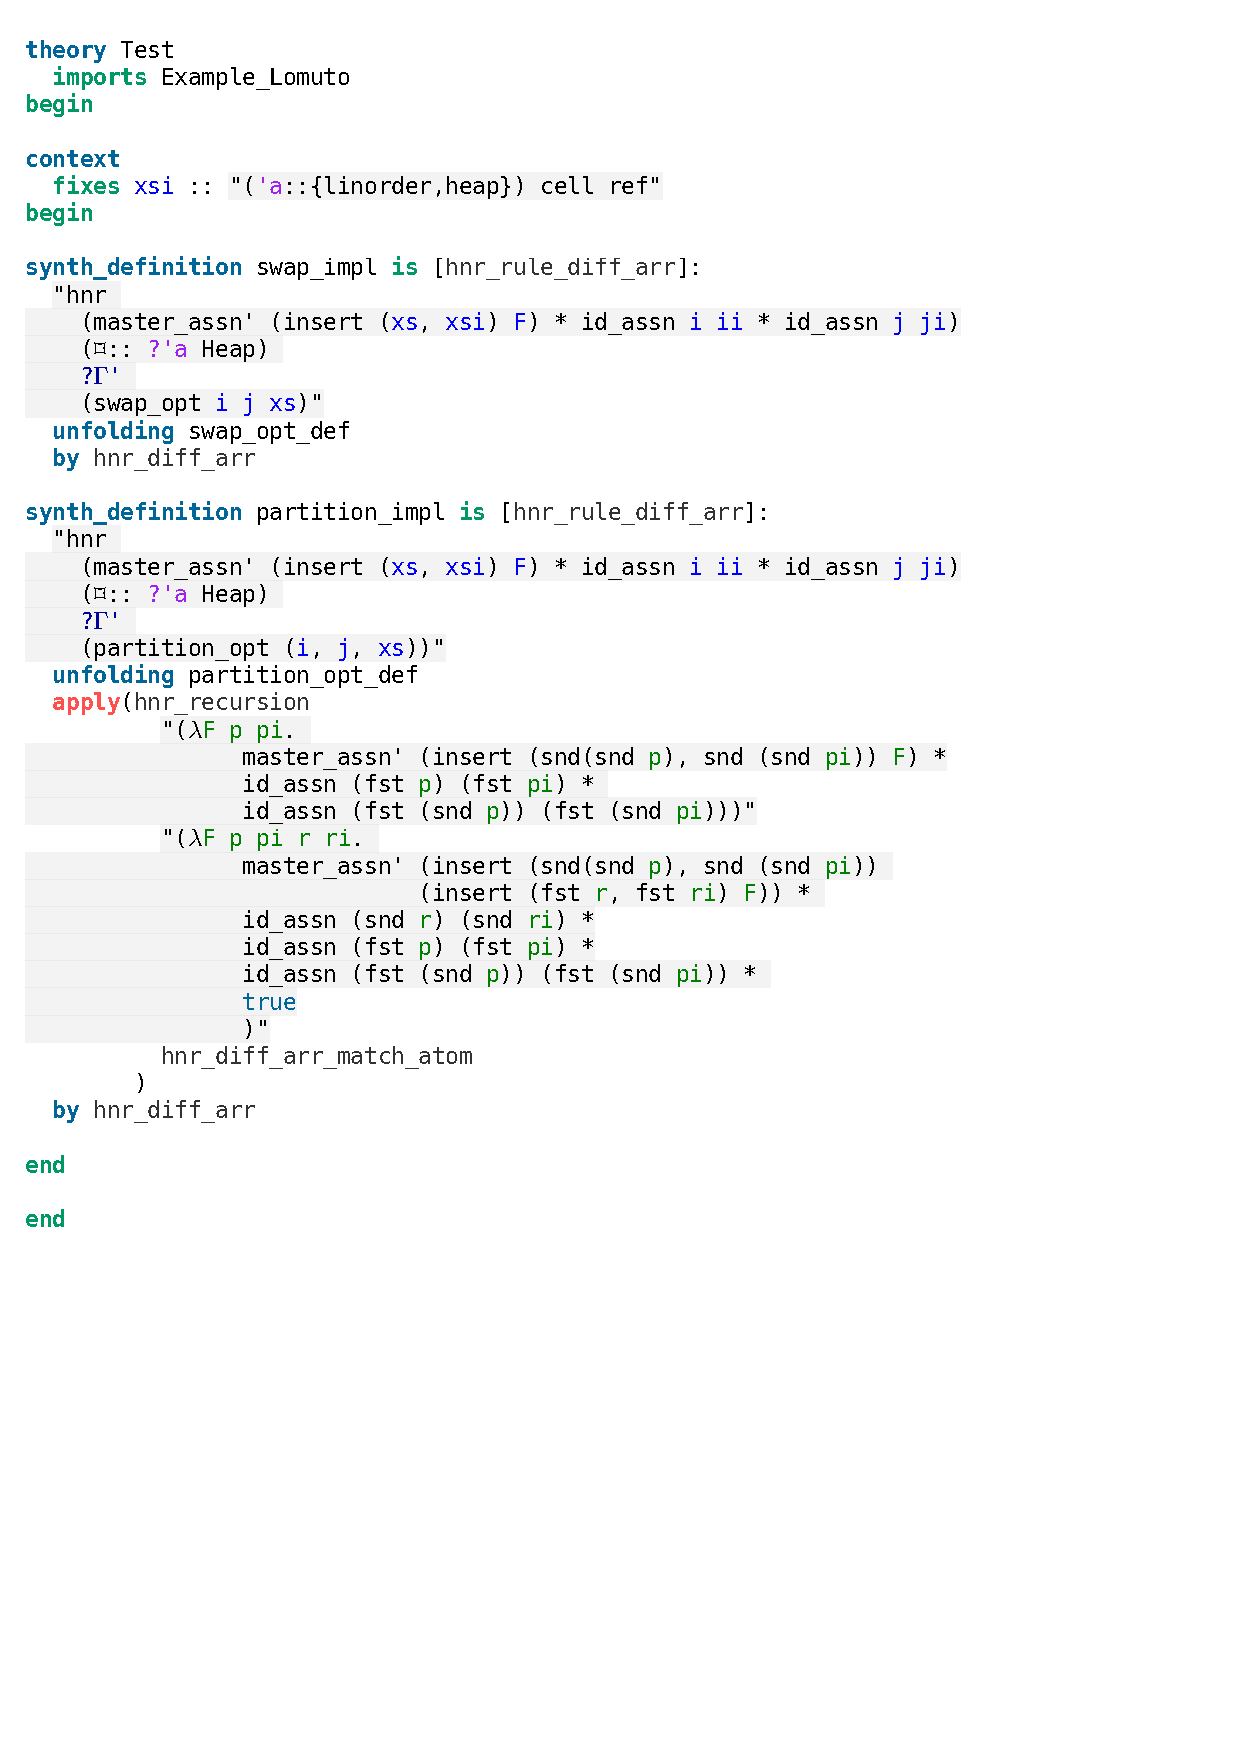
\includegraphics[trim={0 10,6cm 0 4,2cm}, clip, width=1.00\textwidth]{figures/Theory_Example_Lomuto_Translation2.pdf}
    \caption[Refinement of the naive Lomuto partitioning]{Refinement of the naive Lomuto partitioning}
    \label{fig:lomuto_ref}
\end{figure}
